\documentclass[pdf]{beamer}
\mode<presentation>{}

\usepackage[utf8]{inputenc}

\usepackage[sans]{dsfont}
\usepackage{amsmath}

\newcommand{\op}[1]{\operatorname{#1}}
\newcommand{\bbf}[1]{\mathds{#1}}
\newcommand{\Z}{\bbf{Z}}

\title{Bernsteinrelationen, der $2$-Kozykel $\bbf{X}$, und der Raum der Orientierungen}
\author{Nicolas A. Schmidt}
\date{}

\begin{document}

%% title frame
\begin{frame}
   \titlepage
\end{frame}

\begin{frame}{Überblick}
\begin{itemize}
   \item<2-> Zentrales Objekt: \textbf{Hecke-Algebren} \pause[3](Iwahori-Hecke-Algebren, affine Hecke-Algebren, pro-$p$-Iwahori Hecke-Algebren, \dots)\pause[4], genauer \textbf{generische pro$\text{-}p$ Hecke-Algebren}
   \item<5-> Hecke Algebren $\mathcal{H}$ werden gebildet zu
      \begin{itemize}
         \item<6-> einer \textbf{Coxetergruppe}
         \item<7-> und einer \textbf{Familie von Parametern}
      \end{itemize}
   \item<8-> Zentrales Ziel: Bestimmung der Struktur von $\mathcal{H}$\pause[9], insbesondere Bestimmung des \textbf{Zentrums} $Z(\mathcal{H})$
      \pause[10]\[ Z(\mathcal{H}) = \{ z \in \mathcal{H}\ :\ zx = xz\text{ für alle } x \in \mathcal{H} \} \]
   \item<11-> Ideologie:
      \begin{itemize}
         \item<12-> Coxetergruppen sind \textit{geometrische} Objekte
         \item<13-> Verstehe $\mathcal{H}$ vermöge dieser Geometrie!
      \end{itemize}
\end{itemize}
\end{frame}

\begin{frame}{Das einfachste mathematische Objekt}
   \pause
   \begin{figure}
   \centering
      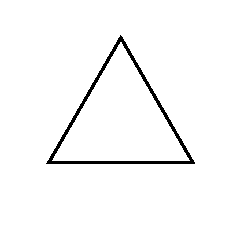
\includegraphics[width=0.5\textwidth]{graphics/triangle.eps}
   \end{figure}
\end{frame}

\end{document}
